\documentclass{article}

\usepackage{hyperref}
\usepackage{listings}
\usepackage{color}
\usepackage[utf8]{inputenc} % usually not needed (loaded by default)
\usepackage[T1]{fontenc}
\usepackage{verbatimbox}
\usepackage{readarray}
\usepackage{amsmath,amssymb}
\usepackage{graphicx}
\usepackage{makeidx}
\usepackage{index}
\usepackage{hyperref}
\usepackage{array}
\usepackage{tikz}
\usepackage{pgfplots}
\pgfplotsset{compat=1.18}
\hypersetup{
  colorlinks=true,
  linkcolor=blue,
  urlcolor=black,
  citecolor=black
}
\makeindex

% Margins
\topmargin=-0.45in
\evensidemargin=0in
\oddsidemargin=0in
\textwidth=6.5in
\textheight=9.0in
\headsep=0.25in

\title{ Introduction to Natural Language Processing, Assignment 2 }
\author{ Enrique Mesonero Ronco \and Sergio Sánchez García \and Ismael Cross Moreno }
\date{\today}

\begin{document}
\maketitle
\begin{figure}[h!]
	\includegraphics[width=\linewidth]{C:/Users/Enrique/Desktop/Clases/Introduction to NLP/Ejercicio 2/Exercise2.png}
\end{figure}
\newpage
\tableofcontents
\newpage
\section { Distributional Semantics }
	\subsection { Raw Co-occurrence Vectors }
Given the following raw co-occurrence counts of words with contexts jealous
$(c_1)$ and gossip $(c_2)$:

	\begin{center}
	\begin{tabular} { | m{2cm} | m{2cm} | m{2cm} | }
		\hline
		 & $c_1 \text{(jealous)}$ &  $c_2 \text{(gossip)} $\\
		\hline
		$w_1$ & 2 & 5 \\
		\hline
		$w_2$ & 3 & 0 \\
		\hline
		$w_3$ & 4 & 0 \\
		\hline
		$w_4$ & 0 & 4 \\
		\hline
	\end{tabular}
	\end{center}

\begin{enumerate}
    \item \textbf{Compute the TF-IDF Weighted Co-occurrence Matrix} \\
    Use the following formulas:
    \[
    \text{tf}(w, c) = \log \left( \frac{\text{freq}(w, c)}{\max_{w'} \text{freq}(w', c)} + 1 \right)
    \]
    \[
    \text{idf}(c) = \log \left( \frac{|V|}{|\{w \in V : \text{freq}(w, c) > 0\}|} \right)
    \]
    Where $|V| = 4$.
\\

    \textbf{TF:}
	\begin{itemize}
	\item $ \text{tf}(w_1, c_1) = \log \left( \frac{2}{4} + 1 \right)=0.176$
	\item $ \text{tf}(w_2, c_1) = \log \left( \frac{3}{4} + 1 \right)=0.243$
	\item $ \text{tf}(w_3, c_1) = \log \left( \frac{4}{4} + 1 \right)=0.301$
	\item $ \text{tf}(w_4, c_1) = \log \left( \frac{0}{4} + 1 \right)=0$
	\item $ \text{tf}(w_1, c_2) = \log \left( \frac{5}{5} + 1 \right)=0.301$
	\item $ \text{tf}(w_2 c_2) = \log \left( \frac{0}{5} + 1 \right)=0$
	\item $ \text{tf}(w_3, c_2) = \log \left( \frac{0}{5} + 1 \right)=0$
	\item $ \text{tf}(w_4, c_2) = \log \left( \frac{4}{5} + 1 \right)=0.255$
	\end{itemize}

    \textbf{IDF:}
	\begin{itemize}
	\item $\text{idf}(c_1)=\log(\frac{4}{3})=0.125$
	\item $\text{idf}(c_2)=\log(\frac{4}{2})=0.301$
	\end{itemize}

\textbf{TF-IDF}
	\begin{itemize}
	\item $ \text{tf-idf}(w_1, c_1) = 0.176 \cdot 0.125 = 0.022$
	\item $ \text{tf-idf}(w_2, c_1) = 0.243 \cdot 0.125 = 0.030$
	\item $ \text{tf-idf}(w_3, c_1) = 0.301 \cdot 0.125 = 0.0376$
	\item $ \text{tf-idf}(w_4, c_1) = 0 \cdot 0.125 = 0$
	\item $ \text{tf-idf}(w_1, c_2) = 0.301 \cdot 0.301 = 0.0906$
	\item $ \text{tf-idf}(w_2, c_2) = 0 \cdot 0.301 = 0$
	\item $ \text{tf-idf}(w_3, c_2) = 0 \cdot 0.301 = 0$
	\item $ \text{tf-idf}(w_4, c_2) = 0.255 \cdot 0.301 = 0.077$
	\end{itemize}
    \item \textbf{Represent Each Word as a TF-IDF Vector}

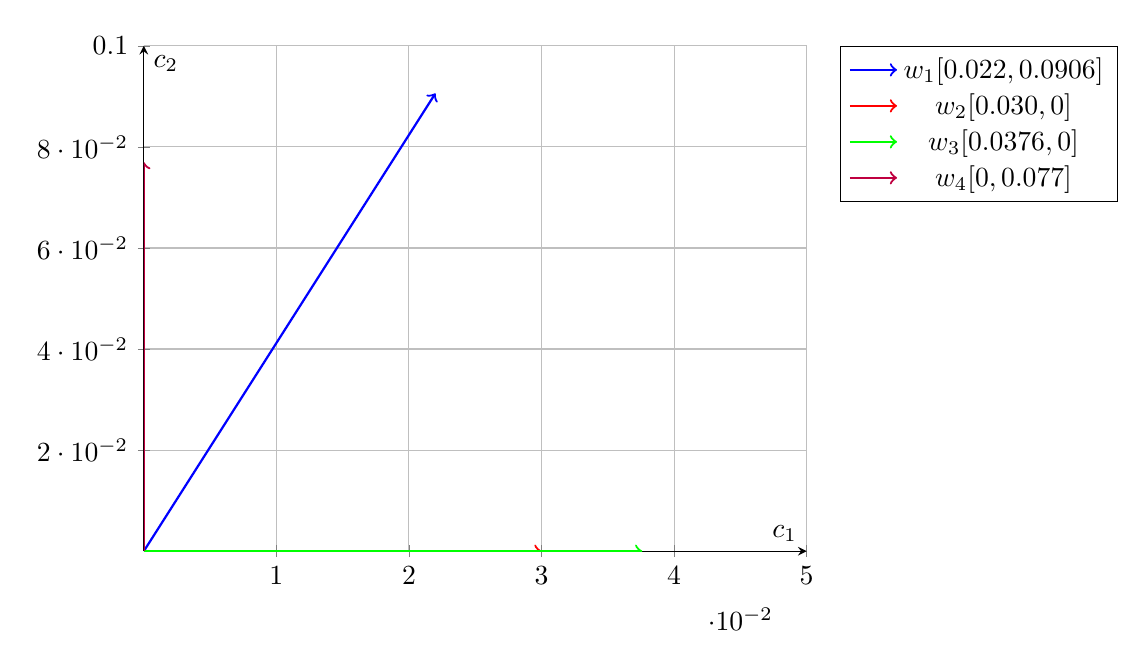
\begin{tikzpicture}
    \begin{axis}[
        axis lines=middle,
        xlabel={$c_1$},
        ylabel={$c_2$},
        xmin=0, xmax=0.05,
        ymin=0, ymax=0.1,
        xtick={0,0.01,0.02,0.03,0.04,0.05},
        ytick={0,0.02,0.04,0.06,0.08,0.1},
        grid=both,
        width=10cm,
        height=8cm,
        legend style={at={(1.05,1)}, anchor=north west},
    ]
    
    % Vector w1
    \addplot[->, thick, color=blue] coordinates {(0,0) (0.022,0.0906)};
    \addlegendentry{$w_1 [0.022, 0.0906]$}
    
    % Vector w2
    \addplot[->, thick, color=red] coordinates {(0,0) (0.030,0)};
    \addlegendentry{$w_2 [0.030, 0]$}
    
    % Vector w3
    \addplot[->, thick, color=green] coordinates {(0,0) (0.0376,0)};
    \addlegendentry{$w_3 [0.0376, 0]$}
    
    % Vector w4
    \addplot[->, thick, color=purple] coordinates {(0,0) (0,0.077)};
    \addlegendentry{$w_4 [0, 0.077]$}
    
    \end{axis}
\end{tikzpicture}

    \item \textbf{Compute the Euclidean Distance Between:}
\[
d(x,y) = \sqrt{\sum_{i=1}^n (x_i - y_i)^2}
\]

    \begin{enumerate}
        \item $w_1$ and $ w_2 \rightarrow 
	d(w_1, w_2) = \sqrt{(0.022 - 0.030)^2 + (0.0906 - 0)^2} = 0.091$
        \item $w_2 $ and $ w_3 \rightarrow
	d(w_1, w_2) = \sqrt{(0.0307 - 0.0376)^2 + (0 - 0)^2} = 0.0076$
    \end{enumerate}
    
    \item \textbf{Discussion} \\
    Based on the Euclidean distances computed, evaluate whether Euclidean distance is an appropriate measure for capturing the relationships between the words.\\
	\textbf{Answer:} Is not a valid option because the Euclidean Distance is affected by vectors length.
\end{enumerate}
	\subsection { Prediction Based Word Vectors }

	\begin{itemize}
		\item Why does Word2Vec use separate input vectors $(u_w)$ and output vectors
$(v_w)$ for each word, and how does this benefit the model’s performance?\\
\textbf{Answer:} Two random vectors (of dimension $d << |V|$) assigned to each word:
		\begin{itemize}
			\item $u_w \rightarrow$ the "input" vector of the word $w$, when it is used to predict another word.
			\item $v_w \rightarrow$ the "output" vector of the word $w$, when it is the one being predicted.
		\end{itemize}

		\item What are the primary differences between the Skip-Gram and Continuous
Bag-of-Words (CBOW) models in Word2Vec, and in what scenarios might
one outperform the other?\\
\textbf{Answer:}
		\begin{itemize} 
			\item Skip-Gram predicts each context words from the center word. More efficient with less amounts of data.
		       	\item CBOW predicts the center word from the whole context. Faster, more efficient with big amounts of data.
		\end{itemize}

		\item How does negative sampling improve the efficiency of training Word2Vec
models compared to using the full softmax function?\\
\textbf{Answer:} Denominator in softmax sums over words in $V_N$, instead of the whole $V \rightarrow N<<|V|$

		\item How does the choice of window size in Word2Vec affect the type of semantic
relationships the model captures?\\
\textbf{Answer:}
		\begin{itemize}
			\item Small windows $\rightarrow$ more sintactic relationships catched
			\item Big windows $\rightarrow$ more semantic relationships catched
		\end{itemize}

		\item What strategies canWord2Vec employ to handle out-of-vocabulary (OOV)
words, and what are the implications of these strategies?\\
\textbf{Answer:} Tokenization: enrich word embeddings with subword information (low frequency "token" and "ization" more frequent). Learn subwords vectors (char n-grams) along with word-level embeddings.
	\end{itemize}

\newpage
\section { Topic Modeling }
Consider a simple corpus with the following characteristics:

\begin{itemize}
    \item \textbf{Vocabulary (V)}: \{apple, banana, cherry\}
    \item \textbf{Number of Topics (K)}: 2
    \item \textbf{Number of Documents (M)}: 2
\end{itemize}

The initial topic distributions over words ($\phi_k$) and document distributions over topics ($\theta_m$) are randomly initialized as follows:

\[
\phi_1 =
\begin{bmatrix}
\frac{1}{3} \frac{1}{3} \frac{1}{3}
\end{bmatrix}, \quad
\phi_2 =
\begin{bmatrix}
\frac{1}{3} \frac{1}{3} \frac{1}{3}
\end{bmatrix}
\]

\[
\theta_1 =
\begin{bmatrix}
\frac{1}{2}  \frac{1}{2}
\end{bmatrix}, \quad
\theta_2 =
\begin{bmatrix}
\frac{1}{2} \frac{1}{2}
\end{bmatrix}
\]

\subsection*{Documents}
\begin{itemize}
    \item \textbf{Document 1}: apple, banana
    \item \textbf{Document 2}: banana, cherry
\end{itemize}

\section*{Steps to Solve}

\subsection*{1. Compute Topic Assignment Probabilities}
For each word in each document, compute the probability of assigning it to each topic using the current $\phi$ and $\theta$ values. Specifically, calculate:
\[
P(z_{mn} = k) \propto \phi_k[w] \times \theta_m[k]
\]
for each word $w$ in document $m$.

The probability of assigning each word \( w \) in document \( m \) to topic \( k \) is calculated as:
\[
P(z_{mn} = k) \propto \phi_k[w] \cdot \theta_m[k]
\]

For both topics (\( k = 1, 2 \)), and all words in the documents:
\[
\phi_k[w] = \frac{1}{3}, \quad \theta_m[k] = \frac{1}{2}
\]
Thus:
\[
P(z_{mn} = k) \propto \frac{1}{3} \cdot \frac{1}{2} = \frac{1}{6}
\]

\subsubsection*{Normalization of \( P(Z_{11} = k) \)}

Given:
\[
P(Z_{11} = 1) \propto \frac{1}{6}, \quad P(Z_{11} = 2) \propto \frac{1}{6}
\]

The sum of unnormalized probabilities is:
\[
\text{Sum} = \frac{1}{6} + \frac{1}{6} = \frac{2}{6}
\]

Normalized probabilities:
\[
P(Z_{11} = 1) = \frac{\frac{1}{6}}{\frac{2}{6}} = \frac{1}{2}
\]
\[
P(Z_{11} = 2) = \frac{\frac{1}{6}}{\frac{2}{6}} = \frac{1}{2}
\]

Thus, both probabilities are:
\[
P(Z_{11} = 1) = \frac{1}{2}, \quad P(Z_{11} = 2) = \frac{1}{2}
\]
The probabilities for all words are equal, so no preference exists between topics.

\subsection*{2. Assign New Topics}
Based on the probabilities computed earlier, assign a new topic to each word in each document. Assume you sample deterministically by choosing the topic with the higher probability.

Since the probabilities are equal, we assign topics deterministically:
\begin{itemize}
    \item \textbf{Document 1:} Assign topic 1 to "apple" and topic 2 to "banana".
    \item \textbf{Document 2:} Assign topic 1 to "banana" and topic 2 to "cherry".
\end{itemize}

\subsection*{3. Update Distributions}
Update the $\phi_k$ and $\theta_m$ distributions based on the new topic assignments. Compute the new probabilities:
\[
P(w|k) = \frac{C(w, k)}{\sum_{w'} C(w', k)}
\]
\[
P(k|d) = \frac{C(k, d)}{\sum_{k'} C(k', d)}
\]
where $C(w, k)$ is the count of word $w$ assigned to topic $k$ across all documents, and $C(k, d)$ is the count of topic $k$ in document $d$.
\textbf{Updated \( \phi_k \):}
\[
P(w|k) = \frac{C(w, k)}{\sum_{w'} C(w', k)}
\]
\[
C(w, k):
\begin{aligned}
    &C(\text{apple}, 1) = 1, \quad C(\text{banana}, 1) = 1, \quad C(\text{cherry}, 1) = 0 \\
    &C(\text{apple}, 2) = 0, \quad C(\text{banana}, 2) = 1, \quad C(\text{cherry}, 2) = 1
\end{aligned}
\]

\[
\phi_1 =
\begin{bmatrix}
\frac{1}{2} % apple
\frac{1}{2} % banana
0            % cherry
\end{bmatrix}, \quad
\phi_2 =
\begin{bmatrix}
0             % apple
\frac{1}{2}  % banana
\frac{1}{2}  % cherry
\end{bmatrix}
\]

\textbf{Updated \( \theta_m \):}
\[
P(k|d) = \frac{C(k, d)}{\sum_{k'} C(k', d)}
\]
\[
C(k, d):
\begin{aligned}
    &C(1, \text{Doc 1}) = 1, \quad C(2, \text{Doc 1}) = 1 \\
    &C(1, \text{Doc 2}) = 1, \quad C(2, \text{Doc 2}) = 1
\end{aligned}
\]

\[
\theta_1 =
\begin{bmatrix}
\frac{1}{2}  % Topic 1
\frac{1}{2}  % Topic 2
\end{bmatrix}, \quad
\theta_2 =
\begin{bmatrix}
\frac{1}{2}  % Topic 1
\frac{1}{2}  % Topic 2
\end{bmatrix}
\]

\end{document}